\documentclass{beamer}
\setbeamertemplate{navigation symbols}{}

\usepackage{beamerthemeshadow}
\usepackage{caption}
\captionsetup{font=scriptsize,labelfont=scriptsize}
\setbeamertemplate{caption}[numbered]

\hypersetup{colorlinks}

\def\gw#1{gravitational wave#1 (GW#1)\gdef\gw{GW}}
\def\ns#1{neutron star#1 (NS#1)\gdef\ns{NS}}

\newcommand{\red}[1]{{\color{red}{#1}}}

\begin{document}

\begin{frame}
    \frametitle{James A. Clark: Gravitational Wave Data Analysis}

    %\begin{itemize}
        %\item 
            {\small `Burst' (unmodelled) GW searches and astrophysical inferences
            through machine learning and Bayesian model selection/parameter
        estimation in ground-based GW detector data.}
    %\end{itemize}

    \begin{columns}[]
        \column{0.5\textwidth}

        \begin{center}
            \vspace{-0.65cm}
            \begin{figure}
                %\scalebox{0.25}{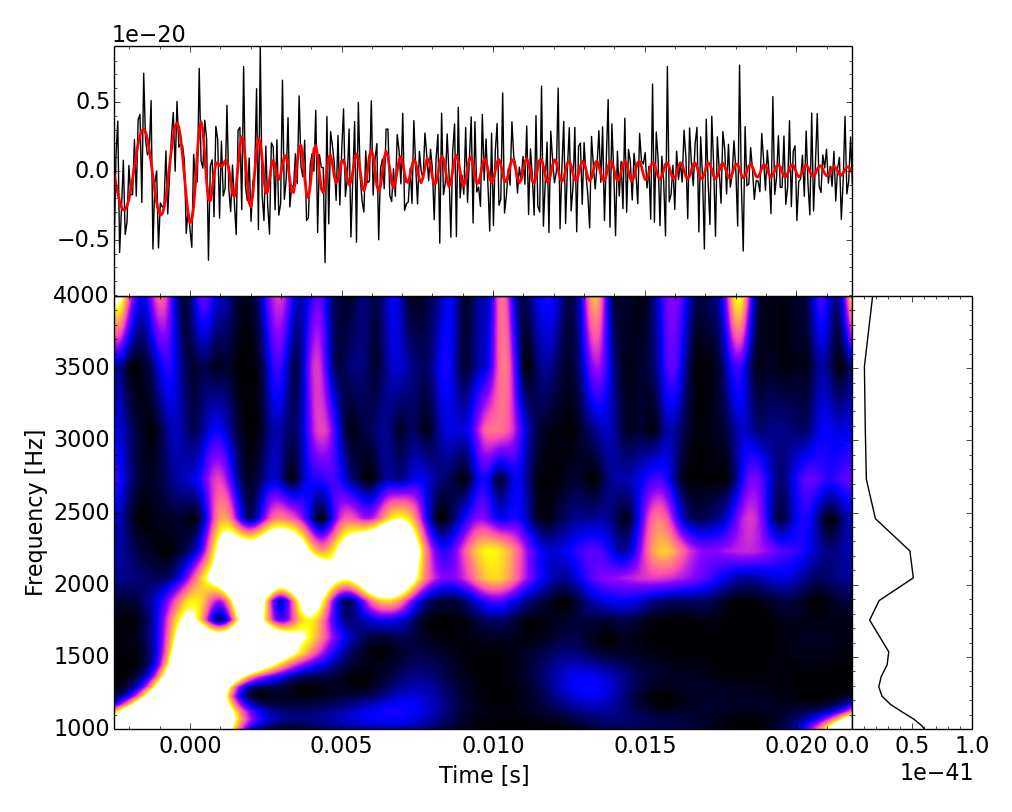
\includegraphics{example_map.png}} \\
                \scalebox{0.35}{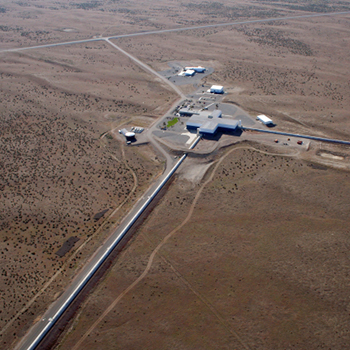
\includegraphics{lho4s.jpg}} \\
                \caption{LIGO Hanford, WA}
            \end{figure}
        \end{center}


        \column{0.6\textwidth}

        \begin{center}
%            \vspace{-.00cm}
            \begin{figure}
                %\scalebox{0.35}{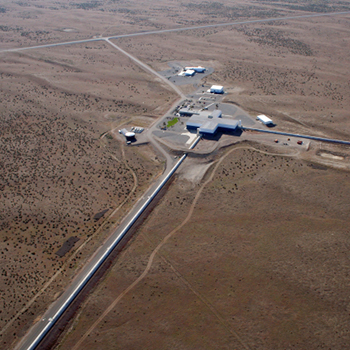
\includegraphics{lho4s.jpg}} \\
                \scalebox{0.25}{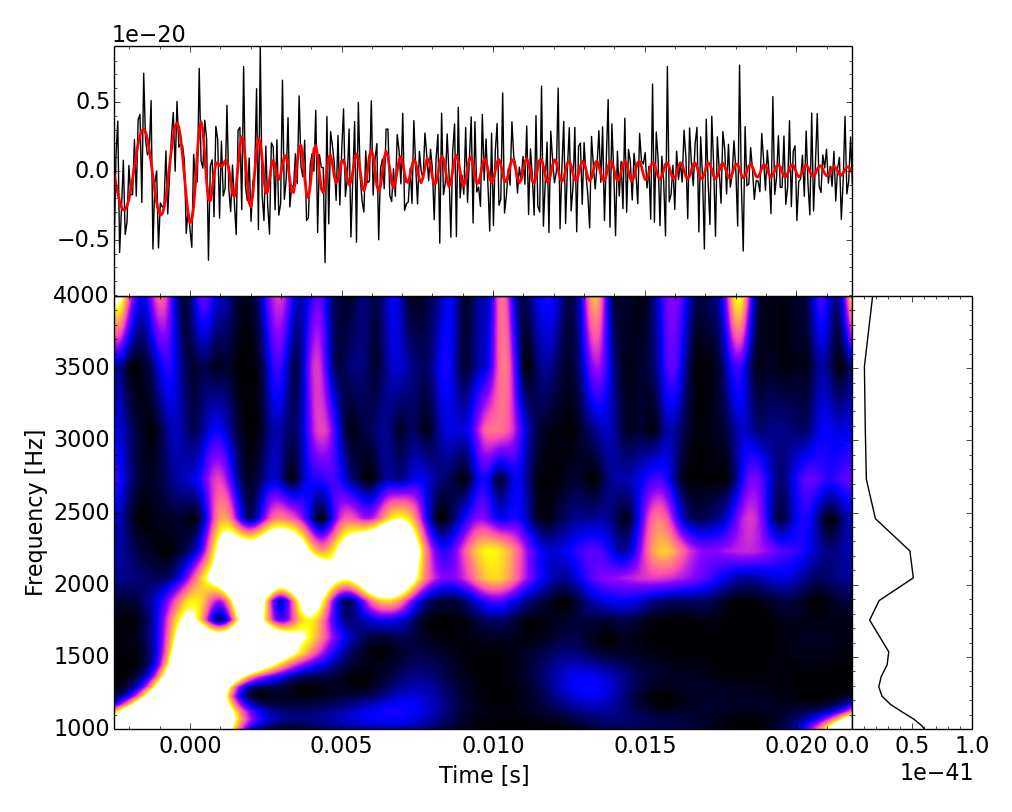
\includegraphics{example_map.png}} \\
                \caption{Example time-frequency map for GW `burst' from
                binary neutron star coalescence in noise}
            \end{figure}
        \end{center}

    \end{columns}


\end{frame}





\end{document}
